\documentclass[oneside, 10pt]{book}
% oneside ist für den Entwurf praktisch. Es schaltet ab, dass 
% Kapitel immer auf der rechten Seite beginnen müssen 
% (und Ähnliches).
%
% Sie setzen die Basisschriftgröße für eine normale Zeile. 
% LaTeX passt den Rest (Überschriften, etc.) daran an.
%
% Die Option draft ersetzt Bilder durch Rahmen 
% und markiert übervolle Zeilen.

\usepackage[utf8]{inputenc} % so ist die Datei encodiert
\usepackage[T1]{fontenc} % verhindert, dass Umlaute bei Copy-n-Paste zu zwei Buchstaben werden

\usepackage[a4paper]{geometry} 
% geometry für Seitenränder, Abstände aller Art, Papierformat, ...

% MATHE
\usepackage{amsmath}
\usepackage{amssymb}


% Blindtext erzeugen um floats et cetera vorführen zu können.
\usepackage{blindtext}


\usepackage[french,english,ngerman]{babel}
% Die zuletzt geladene Sprache wird Default für das Dokument.
% Hier also ngerman (Deutsch neuer Rechtschreibung).
% Sprachwechsel im Text mit \foreignlanguage{}{}.

\usepackage{graphicx} % Bilder einbinden

\usepackage{float}
 % Option H: erzwingt hier!

\usepackage{booktabs} % schöne Tabellen

\usepackage{lmodern}
% Hier setzen wir lmodern als Schrift für das Dokument.

\usepackage{hyperref}
% Verlinkung im Dokument
% Weblinks

\hyphenation{Binnen-schiff-fahrts-kapitäns-patent Boden-schleif-maschinen-verleih}
% Sie können Worttrennungen für das ganze Dokument hier hinterlegen.
% Bei mehrsprachigen Dokumenten beachten Sie die Antwort von egreg hier:
% https://tex.stackexchange.com/questions/182569/how-to-manually-set-where-a-word-is-split


\begin{document}

% automatisch generierte Verzeichnisse:
\tableofcontents % Inhaltsverzeichnis: erfasst Kapitel, Abschnitte, ...
\listoffigures % erfasst alle Bilder, die als figure eingebunden sind
\listoftables % erfasst alle Tabellen, die mit der table Umgebung eingebunden sind.


% Jedes Kapitel in eine eigene Datei.
% Die Dateien brauchen keine Präambel / müssen keine Packages laden.
% Übersetzt nach PDF wird aus dieser Hauptdatei.
% => plus an Übersicht
% => erleichtert die Fehlersuche

\section{Einleitung}

\blindtext
\section{Mathematik}\label{sec:mathe}

Mittels \verb|S formel S| können Sie Formeln in den Fließtext einfügen. Dabei wird eine Formel wie 
$\sum_{i = 0}^{12} = \frac{\sqrt[3]{x^2}}{\pi}$ gestaucht.\\
\ \\
Um eine Formel im abgesetzten Modus anzuzeigen, verwenden Sie \verb|\[ formel \]|. Die Formel wird in einer 
eigenen Zeile angezeigt, aber nicht nummeriert. Also zum Beispiel \[ \cancelto{bla}{\sum_i^5 \sqrt[3]{\pi^2}} \] ohne Nummer.\\
\ \\
Besonders wichtige Formeln sollten Sie nummerieren und mit einem label versehen. So können Sie sich darauf beziehen. Dazu 
müssen Sie die equation-Umgebung nutzen. Beispiel:

\begin{equation}
\left( \int_{\underline{\theta}_b}^{\overline{\theta}_b} Q_b(s) ds\right) \underbrace{F_b}_{= 1} (\overline{\theta}_b) - \left( \int_{\underline{\theta}_b}^{\underline{\theta}_b} Q_b(s) ds\right) \underbrace{F_b(\theta_b}_{0} - \int_{\underline{\theta}_b}^{\overline{\theta}_b} F_b(\theta_b) Q_b(\theta_b) d\theta_b
\label{meineFormel}
\end{equation}

\chapter{Fazit}

\section{Beispiel für floats}

Zum Thema Platzierung von floats, sehen Sie sich bitte diese Seite an:\\
\url{https://tex.stackexchange.com/questions/39017}\\
\ \\
Hier erhalten beide floats die Platzierungsanweisung p und werden erwartungsgemäß beide auf eine gemeinsame Seite verschoben.

\Blindtext

% Ein Bild als figure:
% * es taucht im Bilderverzeichnis auf.
% * Sie können eine Bildunterschrift / caption vergeben.
% * Ein Kurztitel ist möglich.
% Sie können Präferenzen vergeben, wo das Bild angezeigt werden soll.
% Die Reihenfolge hat kein Gewicht, aber das Fehlen einer Option:
% h = here
% t = top of page
% b = bottom of page
% p = page for images
% H = (wenn float geladen ist) Anzeige hier erzwingen
\begin{figure}[p]
\centering
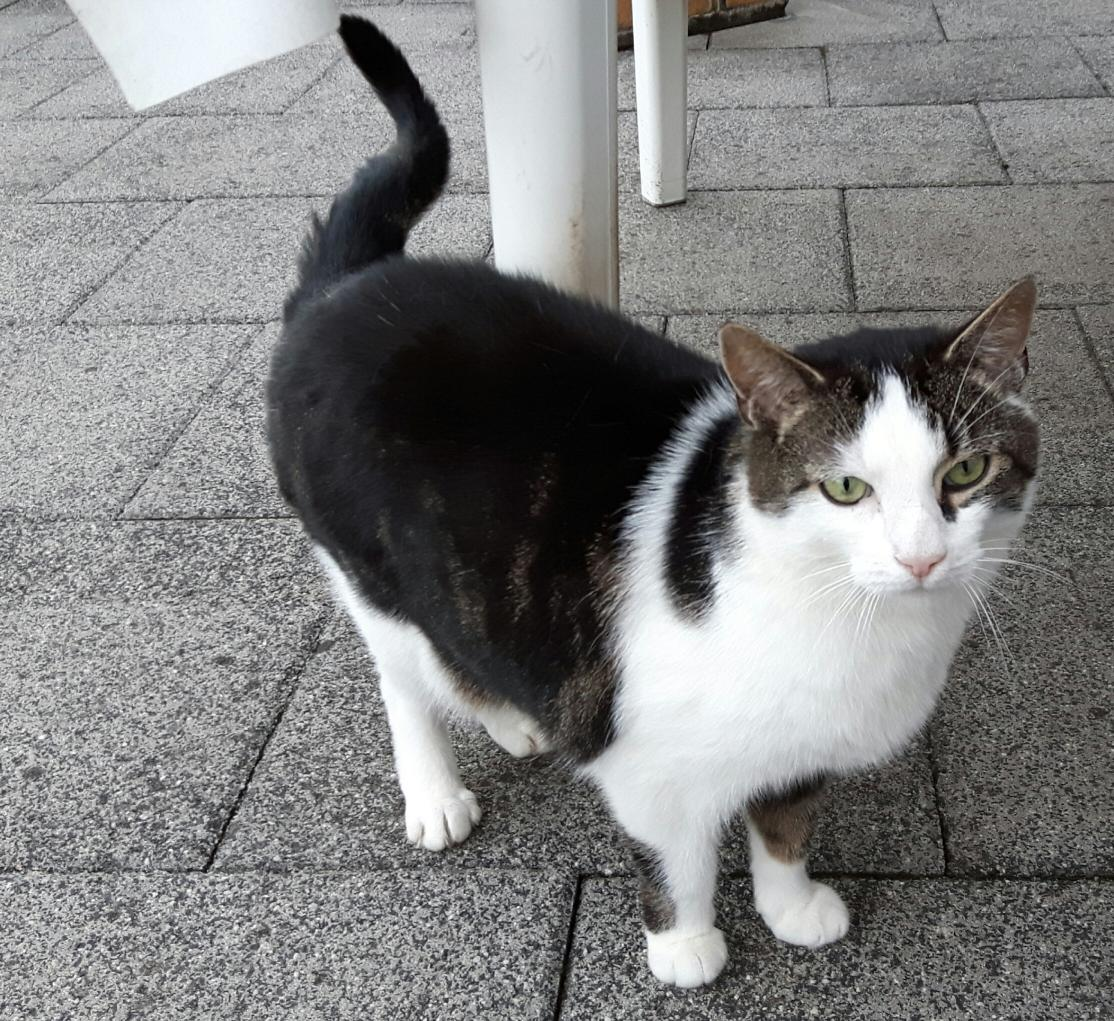
\includegraphics[scale=0.5]{img/Dala}
\label{figDala}
\caption[Kurztitel Katze]{Das ist die Katze Dala im Jahr 2018.}
\end{figure}

\Blindtext

\begin{figure}[p]
\centering
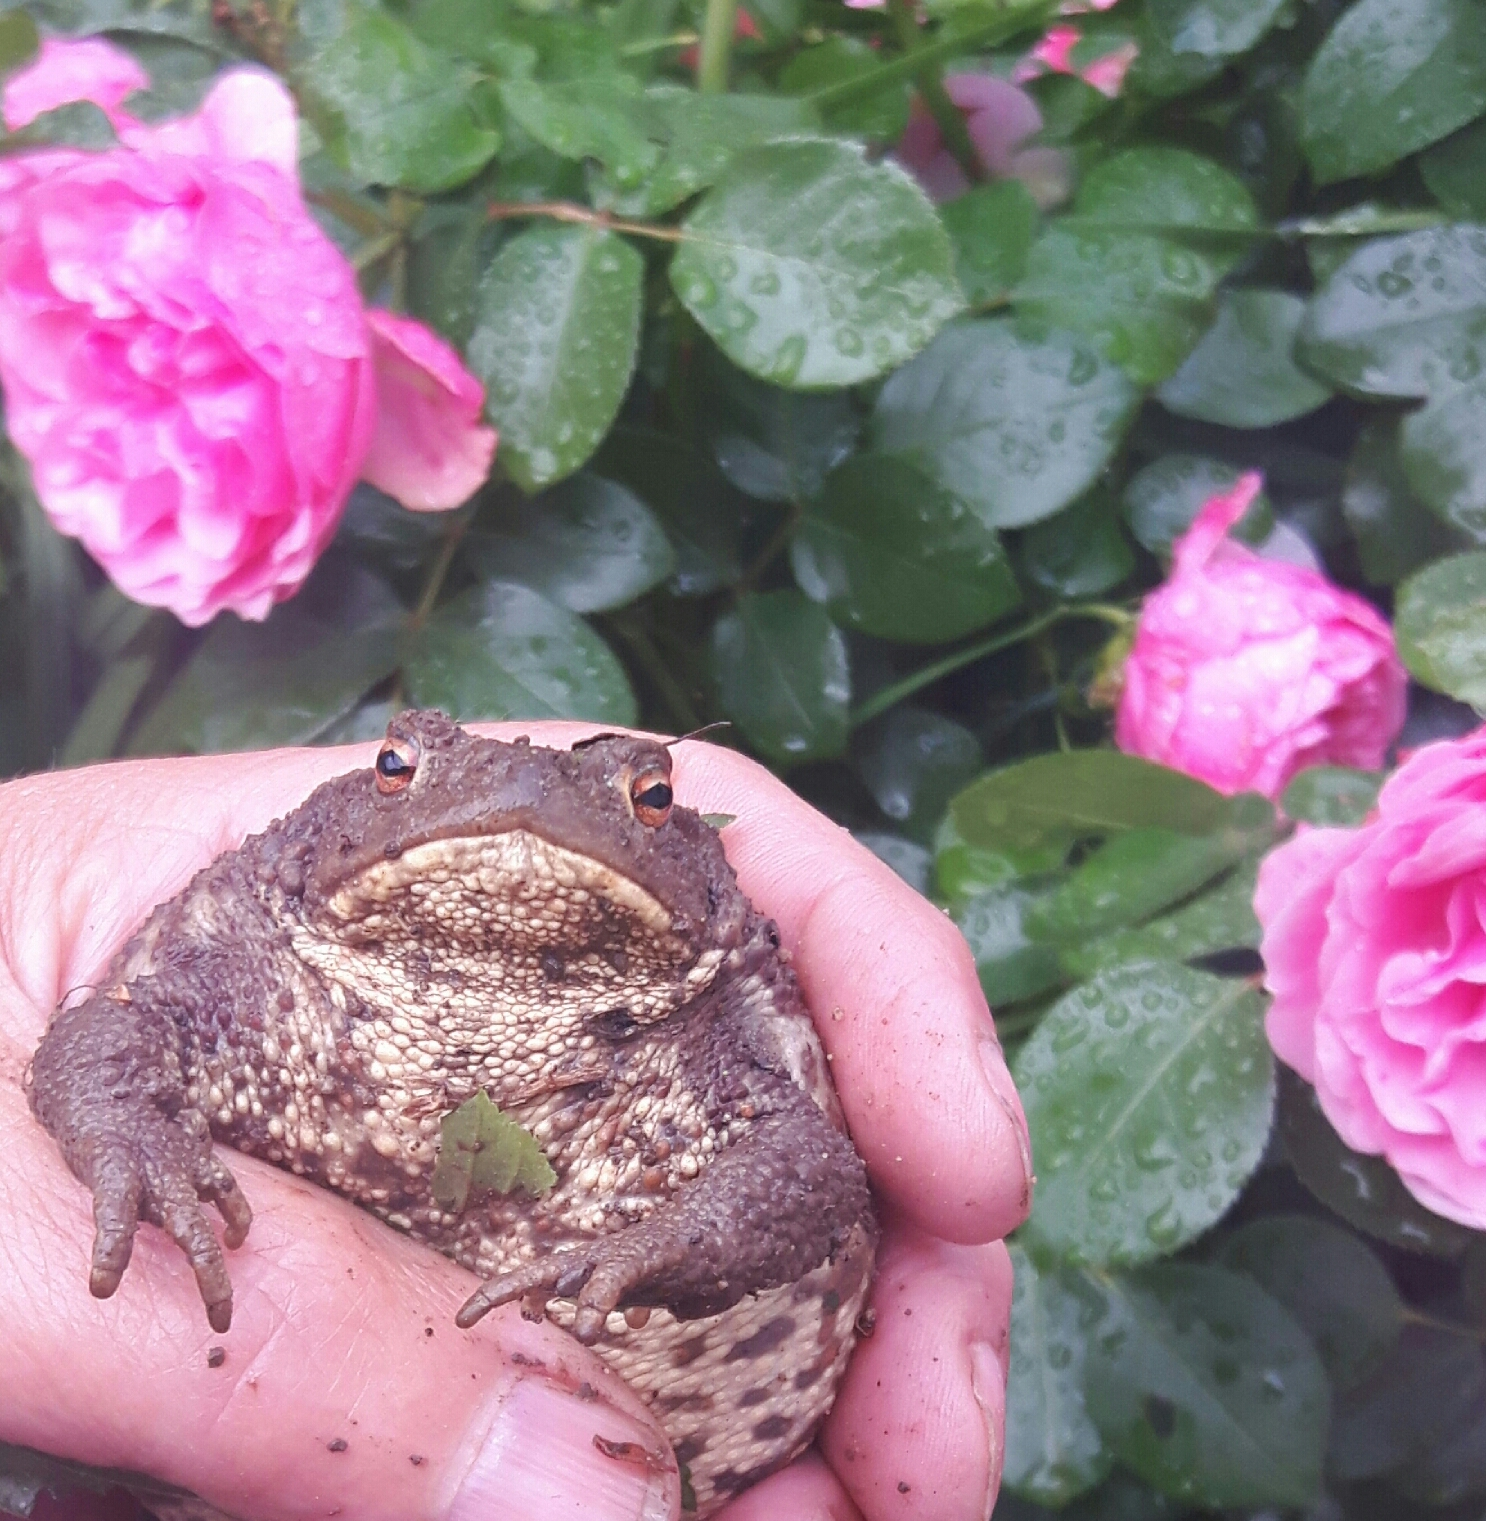
\includegraphics[width=0.4\textwidth]{img/toad}
\label{kroete}
\caption[Kurztitel Kröte]{Kröte, die sich in meinen Garten verirrt hat und zum nächsten Teich gebracht wurde.}
\end{figure}

\Blindtext




\section{Aufzählungen}

Aufzählungen sind eigene Umgebungen und lassen sich schachteln:

\begin{itemize}
\item abc
\item def  \begin{enumerate}
\item eins
\item zwei
\end{enumerate}
\end{itemize}






\url{http://www.uni-koeln.de}



\end{document}